% Source: graduate-coursework/Research/Intro_to_Agents/handouts/Part4_Planning_Workflow.tex

\documentclass[border=4pt]{standalone}
\usepackage{graphicx}
\usepackage{tikz}
\usepackage{xcolor}
\usetikzlibrary{shapes.geometric, arrows.meta, positioning, calc, fit, backgrounds}

\definecolor{UofSCGarnet}{HTML}{73000A}
\definecolor{UofSCBlack}{HTML}{000000}
\definecolor{UofSCWhite}{HTML}{FFFFFF}
\definecolor{UofSCAtlantic}{HTML}{466A9F}
\definecolor{UofSCCongaree}{HTML}{1F414D}
\definecolor{UofSCHorseshoe}{HTML}{65780B}
\definecolor{UofSCRose}{HTML}{CC2E40}
\definecolor{UofSCDarkGarnet}{HTML}{570008}
\definecolor{UofSC90Black}{HTML}{363636}
\definecolor{UofSC70Black}{HTML}{5C5C5C}
\definecolor{UofSC50Black}{HTML}{A2A2A2}

\tikzset{
    box/.style={
        draw=UofSCBlack,
        fill=#1,
        minimum width=2.5cm,
        minimum height=0.8cm,
        text=UofSCWhite,
        font=\small\bfseries,
        align=center,
        inner sep=4pt
    },
    box/.default=UofSCGarnet,
    lightbox/.style={
        draw=UofSCBlack,
        fill=UofSCWhite,
        minimum width=2.5cm,
        minimum height=0.8cm,
        text=UofSCBlack,
        font=\small,
        align=center,
        inner sep=4pt
    },
    arrow/.style={
        ->,
        >=Stealth,
        thick,
        UofSCBlack
    },
    bigarrow/.style={
        ->,
        >=Stealth,
        line width=1.5pt,
        UofSCGarnet
    },
    phase/.style={
        draw=UofSCBlack,
        fill=#1,
        minimum width=3cm,
        minimum height=1cm,
        text=UofSCWhite,
        font=\bfseries,
        align=center
    },
    phase/.default=UofSCGarnet,
    subphase/.style={
        draw=UofSC70Black,
        fill=UofSCWhite,
        minimum width=2.8cm,
        minimum height=0.6cm,
        text=UofSCBlack,
        font=\scriptsize,
        align=center
    },
    cyclebox/.style={
        draw=UofSCBlack,
        line width=1.5pt,
        fill=#1,
        minimum width=2cm,
        minimum height=1.2cm,
        text=UofSCWhite,
        font=\bfseries,
        align=center
    },
    cyclebox/.default=UofSCGarnet
}

\begin{document}
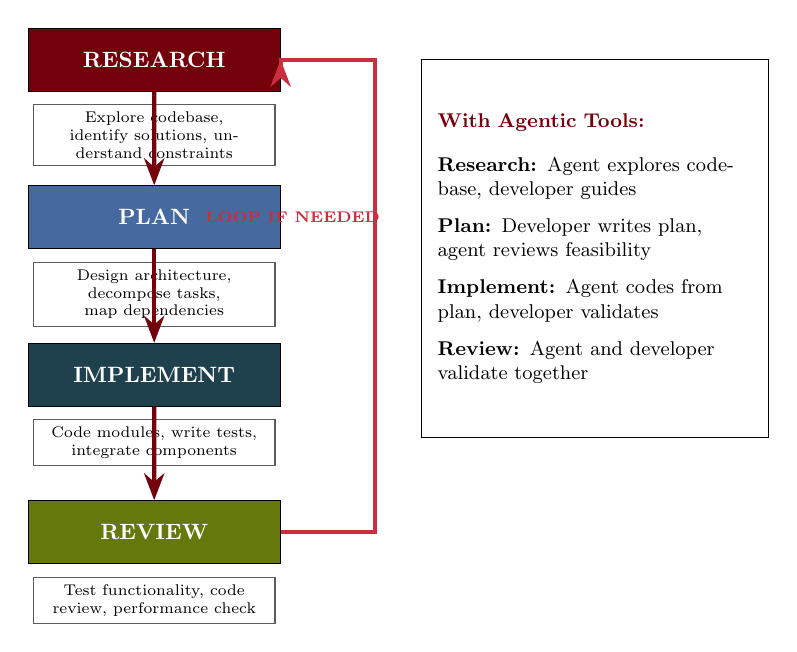
\begin{tikzpicture}[node distance=1.8cm, scale=0.8, transform shape]
        % Research phase
        \node[phase=UofSCGarnet, minimum width=4cm] (research) at (0,3) {RESEARCH};
        \node[subphase, below=0.2cm of research, minimum width=3.8cm, text width=3.6cm] (r1) {Explore codebase, identify solutions, understand constraints};

        % Plan phase
        \node[phase=UofSCAtlantic, minimum width=4cm] (plan) at (0,0.5) {PLAN};
        \node[subphase, below=0.2cm of plan, minimum width=3.8cm, text width=3.6cm] (p1) {Design architecture, decompose tasks, map dependencies};

        % Implement phase
        \node[phase=UofSCCongaree, minimum width=4cm] (impl) at (0,-2) {IMPLEMENT};
        \node[subphase, below=0.2cm of impl, minimum width=3.8cm, text width=3.6cm] (i1) {Code modules, write tests, integrate components};

        % Review phase
        \node[phase=UofSCHorseshoe, minimum width=4cm] (review) at (0,-4.5) {REVIEW};
        \node[subphase, below=0.2cm of review, minimum width=3.8cm, text width=3.6cm] (rev1) {Test functionality, code review, performance check};

        % Arrows
        \draw[bigarrow] (research) -- (plan);
        \draw[bigarrow] (plan) -- (impl);
        \draw[bigarrow] (impl) -- (review);

        % Loop back arrow
        \draw[bigarrow, UofSCRose] (review.east) -- ++(1.5,0) -- ++(0,7.5) -- ++(-1.5,0) -- (research.east);
        \node[text=UofSCRose, font=\scriptsize\bfseries] at (2.2,0.5) {LOOP IF NEEDED};

        % Right side - with agentic tools
        \node[lightbox, minimum width=5.5cm, minimum height=6cm, text width=5cm, align=left] at (7,0) {
            \textbf{\textcolor{UofSCGarnet}{With Agentic Tools:}}\\[0.3cm]
            \textbf{Research:} Agent explores codebase, developer guides\\[0.2cm]
            \textbf{Plan:} Developer writes plan, agent reviews feasibility\\[0.2cm]
            \textbf{Implement:} Agent codes from plan, developer validates\\[0.2cm]
            \textbf{Review:} Agent and developer validate together
        };
    \end{tikzpicture}
\end{document}
